\documentclass[11pt]{article}

% Compatibility for the older MiKTeX kernel installed on this machine.
\providecommand\IfDocumentMetadataTF[2]{#2}

\usepackage[margin=1in]{geometry}
\usepackage{amsmath,amssymb}
\usepackage{array,longtable}
\usepackage{enumitem}
\usepackage{graphicx}
\usepackage[hidelinks]{hyperref}

\newcommand{\E}{\mathbb E}
\newcommand{\Var}{\operatorname{Var}}
\newcommand{\Cov}{\operatorname{Cov}}
\newcommand{\Corr}{\operatorname{Corr}}
\newcommand{\MSE}{\operatorname{MSE}}
\newcommand{\indep}{\mathrel{\perp\!\!\!\perp}}

\title{The Cell-Level Precision Problem in the AI Validation Design}
\author{AI Productivity Project: Current Writeup}
\date{August 4, 2026}

\begin{document}
\maketitle

\section*{Purpose and source convention}

This note asks whether the proposal can estimate the true productivity gain
\(\theta_j\) precisely for a cell that does not receive an RCT. It first
shows why the held-out-cell MSE contains a nonvanishing term \(\omega^2\).
It then reports a reproducible simulation of the MSE as the number of
validated cells grows. Finally, it states what must change if precise
cell-level estimation, rather than calibrated prediction, is the objective.
It also isolates the exact point at which the proposal's interpretation
goes beyond its formal result.

The project source is \textit{The Distributional Effects of AI's Productivity
Gains: A Data Fusion Approach}, especially pp.~2--4. Statements marked
\emph{Source} come from that proposal. Statements marked \emph{Proposal
claim} are asserted there without proof. Statements marked \emph{Assumption}
or \emph{Calibration} are added here. Statements marked \emph{Derived} follow
from displayed assumptions. Statements marked \emph{Simulation result} come
from the program
\texttt{ai\_mse\_simulation\_2026-08-04.py}, archived at commit
\href{https://github.com/michaeljwang6/loo_simulation/commit/4307f84}
{4307f84}.

\section{What is observed and what remains unknown}

\subsection*{Notation}

\begin{longtable}{>{\raggedright\arraybackslash}p{0.24\linewidth}
                  >{\raggedright\arraybackslash}p{0.68\linewidth}}
\hline
Symbol & Meaning \\
\hline
\endfirsthead
\hline
Symbol & Meaning \\
\hline
\endhead
\(j=1,\ldots,J\) & Occupation-task cell and total number of cells. \\
\(R_j,m\) & Validation indicator and number of validated cells,
\(m=\sum_jR_j\). \\
\(\theta_j\) & True productivity gain in cell \(j\). \\
\(S_j\) & Broad model score observed in every cell. \\
\(\widehat v_j,\varepsilon_j,s_j^2\) & RCT estimate in a validated cell,
its error, and its design variance. \\
\(\mu,\tau^2\) & Cross-cell mean and variance of true gains. \\
\(a,b\) & Score intercept and score slope; \(0<b<1\) represents
compression. \\
\(\eta_j,\sigma_S^2\) & Score error and its variance. \\
\(\psi,\psi_0\) & Generic and true shared parameter vectors, ordered as
\((\mu,\tau^2,a,b,\sigma_S^2)\). \\
\(\mathcal D_m\) & Data from the \(m\) validated cells. \\
\(h(S;\psi)\) & Conditional-mean rule evaluated at score \(S\) and shared
parameter \(\psi\). \\
\(m_j\) & Oracle score-only prediction
\(\E[\theta_j\mid S_j,\psi_0]=h(S_j;\psi_0)\). \\
\(u_j\) & Cell-specific difference \(\theta_j-m_j\). \\
\(\omega^2\) & Score-only conditional variance
\(\Var(\theta_j\mid S_j,\psi_0)\), constant in the Gaussian model. \\
\(\widehat\psi_m,\widehat\theta_{j,m}\) & Shared-parameter estimator and
held-out-cell prediction \(h(S_j;\widehat\psi_m)\). \\
\(\mathcal R_m,\Delta_m\) & Held-out-cell MSE and its excess above the
oracle floor. \\
\(\Lambda\) & Constant in the expansion
\(\Delta_m=\Lambda/m+o(m^{-1})\). \\
\(o(m^{-1})\) & A term that is small relative to \(m^{-1}\). \\
\(\sigma_\theta^2,\beta,\nu_j,\widehat\theta_j^v\) & Proposal aliases for
\(\tau^2,b,\eta_j,\widehat v_j\), used only in the conversion below. \\
\hline
\end{longtable}

\noindent\textit{Source-to-project notation conversion.}
The proposal uses \(\sigma_\theta^2,\beta,\nu_j,\widehat\theta_j^v\), while
the project notes use \(\tau^2,b,\eta_j,\widehat v_j\). This note keeps the
project notation. The symbols \(\mathcal D_m,u_j,\mathcal R_m\), and
\(\Delta_m\) are added because the proposal does not name these objects.

The data differ between validated and unvalidated cells:
\begin{center}
\begin{tabular}{p{0.18\linewidth}p{0.27\linewidth}p{0.43\linewidth}}
\hline
Cell & Observed data & Information supplied \\
\hline
\(R_j=1\) & \(S_j,\widehat v_j\) & The score and a noisy direct measurement
of this cell's gain. \\
\(R_j=0\) & \(S_j\) only & The score-to-truth relation learned from other
cells, but no direct measurement of this cell's gain. \\
\hline
\end{tabular}
\end{center}
The proposal uses approximately \(J=1{,}000\) cells and an experimental
anchor of roughly \(m=40\) cells. The MSE curve in Figure~2 is evaluated on
held-out cells. \emph{Source: proposal, pp.~1--3.}

The model for one basket is
\begin{equation}
 \theta_j\sim N(\mu,\tau^2),
 \qquad
 S_j=a+b\theta_j+\eta_j,
 \qquad
 \eta_j\sim N(0,\sigma_S^2),
 \qquad
 \eta_j\indep\theta_j.
 \label{eq:model}
\end{equation}
For a validated cell,
\begin{equation}
 \widehat v_j=\theta_j+\varepsilon_j,
 \qquad
 \varepsilon_j\sim N(0,s_j^2),
 \qquad
 \varepsilon_j\indep(\theta_j,\eta_j).
 \label{eq:validation}
\end{equation}
The Gaussian validation equation is from the proposal. Independence of the
score and validation errors is made explicit here because it is required for
the posterior calculation below. \emph{Source and additional assumption:
proposal, p.~4, translated into project notation.}

Normal updating gives
\begin{align}
 m_j
 &=h(S_j;\psi_0) \\
 &=\mu+
 \frac{b\tau^2}{b^2\tau^2+\sigma_S^2}
 (S_j-a-b\mu),
 \label{eq:oracle-mean}\\
 \omega^2
 &=\Var(\theta_j\mid S_j,\psi_0) \\
 &=\frac{\tau^2\sigma_S^2}{b^2\tau^2+\sigma_S^2}.
 \label{eq:oracle-variance}
\end{align}
\emph{Derived from \eqref{eq:model}.}

Write
\begin{equation}
 \theta_j=m_j+u_j,
 \qquad
 \E[u_j\mid S_j,\psi_0]=0,
 \qquad
 \E[u_j^2\mid S_j,\psi_0]=\omega^2.
 \label{eq:residual}
\end{equation}
The validation sample can learn the distribution of \(u_j\). It does not
reveal the realized \(u_j\) for a cell with \(R_j=0\). Even when
\(\psi_0\) is known, the score equation contains two unknown realized values,
\(\theta_j\) and \(\eta_j\), for one observed \(S_j\).

For the plug-in prediction \(\widehat\theta_{j,m}\), Appendix~A proves the
exact decomposition
\begin{equation}
 \mathcal R_m
 =\E[(\widehat\theta_{j,m}-\theta_j)^2]
 =\omega^2+
 \underbrace{\E[(\widehat\theta_{j,m}-m_j)^2]}_{\Delta_m}.
 \label{eq:main-decomposition}
\end{equation}
Under the regularity conditions in Appendix~A,
\begin{equation}
 \Delta_m=\frac{\Lambda}{m}+o(m^{-1}),
 \qquad
 \mathcal R_m=\omega^2+\frac{\Lambda}{m}+o(m^{-1}).
 \label{eq:main-expansion}
\end{equation}
\emph{Derived.} The proposal asserts the \(m^{-1}\) excess-risk rate but
does not supply its assumptions or proof. \emph{Proposal claim: p.~4,
Appendix A.3.}

The restriction \(R_j=0\) is essential. If \(j\) is validated and the shared
parameters are known, combining \(S_j\) and \(\widehat v_j\) gives
\begin{equation}
 \Var(\theta_j\mid S_j,\widehat v_j,\psi_0)
 =\left(\frac1{\omega^2}+\frac1{s_j^2}\right)^{-1}
 =\frac{\omega^2s_j^2}{\omega^2+s_j^2}.
 \label{eq:validated-variance}
\end{equation}
\emph{Derived from \eqref{eq:model}--\eqref{eq:validation}.} The
\(\omega^2\) floor studied below applies to the cells that the proposal asks
the model to extrapolate to, not to a cell that receives its own precise RCT.

\section{Simulation of MSE as the validation anchor grows}

\subsection*{Notation}

\begin{longtable}{>{\raggedright\arraybackslash}p{0.24\linewidth}
                  >{\raggedright\arraybackslash}p{0.68\linewidth}}
\hline
Symbol & Meaning \\
\hline
\endfirsthead
\hline
Symbol & Meaning \\
\hline
\endhead
\(j,J,m\) & Cell index, total cells, and number of validated cells. \\
\(\theta_j,S_j,\eta_j,\widehat v_j,\varepsilon_j,s_j^2\) & True gain,
broad score, score error, RCT estimate, validation error, and
validation-estimate variance. \\
\(\mu,\tau^2,a,b,\sigma_S^2\) & The five shared Gaussian channel
parameters. \\
\(\psi_0,\widehat\psi_m\) & True and fitted shared parameter vectors. \\
\(h,m_j,\widehat\theta_{j,m}\) & Conditional-mean rule, oracle score-only
prediction, and fitted held-out prediction. \\
\(\omega^2,\mathcal R_m,\Delta_m,\Lambda\) & Oracle floor, total held-out
MSE, excess MSE, and its first-order coefficient. \\
\(\rho\) & Score-truth correlation \(\Corr(S_j,\theta_j)\). \\
\(D_S,\mu_S\) & True score variance
\(b^2\tau^2+\sigma_S^2\) and mean \(a+b\mu\). \\
\(c,\widehat c_m\) & True and fitted conditional-mean slopes,
\(c=b\tau^2/D_S\). \\
\(N_{\rm MC}\) & Number of Monte Carlo repetitions. \\
\(r=1,\ldots,N_{\rm MC}\) & Monte Carlo replication index. \\
\(\mathcal M\) & Simulated validation-budget grid. \\
\(\bar S_m,\overline v_m\) & Validation-sample means of the score and RCT
estimate. \\
\(\widehat V_{S,m},\widehat V_{v,m},\widehat C_{Sv,m}\) & Validation-sample
score variance, RCT-estimate variance, and their covariance. \\
\([x]_+,\Pi_{[0,1]}(x)\) & Numerical projections
\(\max(x,10^{-10})\) and \(\min\{1,\max(0,x)\}\). \\
\(\widehat\mu_m,\widehat\tau_m^2,\widehat a_m,
\widehat b_m,\widehat\sigma_{S,m}^2\) & Moment estimators of the five shared
parameters. \\
\(\widehat\Lambda\) & Coefficient fitted to the simulated relation
\(\Delta_m\simeq\widehat\Lambda/m\). \\
\(\Delta_m^{(r)},\widehat\Delta_m^{\rm MC},
\widehat{\mathcal R}_m^{\rm MC}\) & Integrated excess risk in replication
\(r\), its Monte Carlo mean, and the corresponding total-risk mean. \\
\(\operatorname{MCSE}\) & Monte Carlo standard error of a simulated mean. \\
\hline
\end{longtable}

\subsection*{Calibration}

The proposal says that \(J\) is on the order of one thousand, uses
approximately \(m=40\) validated cells in its illustration, reports a
score-truth correlation near \(0.44\), and illustrates compression with a
slope near \(0.4\). \emph{Source: proposal, pp.~1--3 and p.~5.}
The value on p.~5 is a Spearman correlation. The Gaussian simulation sets the
Pearson correlation \(\rho\) to the same numerical value as an illustrative
calibration; the proposal does not imply that these two correlations are
equal. \emph{Calibration qualification.}

The primary simulation uses
\begin{equation}
 \mu=30,
 \quad
 \tau=10,
 \quad
 b=0.4,
 \quad
 \rho=0.44,
 \quad
 a=(1-b)\mu=18,
 \quad
 s_j=3.
 \label{eq:calibration}
\end{equation}
Gains and standard deviations are in percentage points. The choices
\(\mu=30,\tau=10\), and \(s_j=3\) are illustrative rather than empirical
estimates. \emph{Calibration.}

The score-noise variance is chosen to match \(\rho\):
\begin{align}
 \rho
 &=\frac{b\tau}{\sqrt{b^2\tau^2+\sigma_S^2}}, \\
 \sigma_S^2
 &=b^2\tau^2(\rho^{-2}-1)
 =66.64.
 \label{eq:score-noise-calibration}
\end{align}
Hence \(\sigma_S=8.16\). The oracle floor is
\begin{equation}
 \omega^2
 =\tau^2(1-\rho^2)
 =80.64,
 \qquad
 \sqrt{\omega^2}=8.98.
 \label{eq:simulation-floor}
\end{equation}
\emph{Derived from \eqref{eq:oracle-variance} and the calibration.}

\subsection*{Method}

The simulation uses \(J=1{,}000\), seed 20260804, and
\begin{equation}
 \mathcal M=\{10,20,40,80,160,320,640\}.
 \label{eq:m-grid}
\end{equation}
The value \(m=640\) is included only to display the rate farther along the
curve; it is not part of the proposal's \(m\ll J\) benchmark. For each Monte
Carlo repetition, the simulation performs the following steps. Hatted sample
moments depend on \(r\); that superscript is suppressed inside the steps.

\begin{enumerate}[label=\arabic*.,leftmargin=2.2em]
 \item Draw \(J\) cells from \eqref{eq:model} and draw validation estimates
 from \eqref{eq:validation} with common variance \(s_j^2=9\). The first
 \(m\) cells form a nested validation anchor. Because the cells are
 exchangeable, this is distributionally equivalent to selecting \(m\) cells
 at random.

 \item Estimate the shared channel by the proposal's identifying moments.
 The sample variances and covariance below use denominator \(m-1\):
 \begin{align}
  \widehat\mu_m
  &=\overline v_m, \\
  \widehat\tau_m^2
  &=[\widehat V_{v,m}-s_j^2]_+, \\
  \widehat b_m
  &=\Pi_{[0,1]}
    \left(\frac{\widehat C_{Sv,m}}{\widehat\tau_m^2}\right), \\
  \widehat a_m
  &=\bar S_m-\widehat b_m\widehat\mu_m, \\
  \widehat\sigma_{S,m}^2
  &=[\widehat V_{S,m}-\widehat b_m^2\widehat\tau_m^2]_+.
  \label{eq:simulation-moments}
 \end{align}
 The projections enforce the parameter space only when a small validation
 sample produces invalid raw moments. They are used in 15.3 percent of
 repetitions at \(m=10\), 3.85 percent at \(m=20\), 0.4 percent at
 \(m=40\), and zero repetitions at \(m\geq80\).

 \item Form \(\widehat\psi_m\), calculate
 \(\widehat c_m=\widehat b_m\widehat\tau_m^2/
 (\widehat b_m^2\widehat\tau_m^2+\widehat\sigma_{S,m}^2)\), and predict a
 held-out cell by
 \begin{equation}
  \widehat\theta_{j,m}
  =\widehat\mu_m+\widehat c_m(S_j-\bar S_m).
  \label{eq:simulation-predictor}
 \end{equation}

 \item Integrate over a new held-out score conditional on the fitted rule.
 The exact excess risk in repetition \(r\) is
 \begin{equation}
 \Delta_m^{(r)}
  =\{\widehat\mu_m+\widehat c_m(\mu_S-\bar S_m)-\mu\}^2
   +(\widehat c_m-c)^2D_S.
 \label{eq:integrated-excess}
 \end{equation}
 The reported simulation means are
 \begin{equation}
  \widehat\Delta_m^{\rm MC}
  =\frac1{N_{\rm MC}}\sum_{r=1}^{N_{\rm MC}}\Delta_m^{(r)},
  \qquad
  \widehat{\mathcal R}_m^{\rm MC}
  =\omega^2+\widehat\Delta_m^{\rm MC}.
  \label{eq:mc-risk-means}
 \end{equation}
 This removes evaluation-sample noise but does not replace the simulated
 validation anchor. A separate calculation predicts the remaining
 \(J-m\) cells directly; its mean MSE differs from the integrated risk by at
 most 0.073 MSE units over the simulated grid.

 \item Begin with \(N_{\rm MC}=2{,}000\) repetitions. Increase that number
 only if the largest relative \(\operatorname{MCSE}\) for \(m\geq40\)
 exceeds 3 percent. The run stopped at 2,000 because the largest relative
 \(\operatorname{MCSE}\) was 2.37 percent. A run with 10,000 repetitions was
 therefore unnecessary for the stated accuracy target.
\end{enumerate}

\noindent\emph{Simulation method.} The program uses the code names
\texttt{sigma\_theta} and \texttt{beta} for the project symbols \(\tau\) and
\(b\). All results below are generated by the archived code; none are
proposal estimates.

\subsection*{Results}

\begin{center}
\begin{tabular}{r r r r r}
\hline
\(m\) & \(\widehat\Delta_m^{\rm MC}\) &
\(\widehat{\mathcal R}_m^{\rm MC}\) &
\(m\widehat\Delta_m^{\rm MC}\) &
\(\omega^2/\widehat{\mathcal R}_m^{\rm MC}\) \\
\hline
10  & 19.940 & 100.580 & 199.4 & 80.2\% \\
20  &  9.988 &  90.628 & 199.8 & 89.0\% \\
40  &  5.013 &  85.653 & 200.5 & 94.1\% \\
80  &  2.331 &  82.971 & 186.5 & 97.2\% \\
160 &  1.129 &  81.769 & 180.7 & 98.6\% \\
320 &  0.579 &  81.219 & 185.4 & 99.3\% \\
640 &  0.283 &  80.923 & 180.9 & 99.7\% \\
\hline
\end{tabular}
\end{center}
\emph{Simulation result.} The first risk column estimates the shrinking
shared-parameter term \(\Delta_m\); the second estimates
\(\mathcal R_m=80.64+\Delta_m\).

The fitted relation is
\begin{equation}
 \mathcal R_m\simeq80.64+\frac{196.7}{m}.
 \label{eq:fitted-mse}
\end{equation}
Regressing \(\log\widehat\Delta_m^{\rm MC}\) on \(\log m\) for
\(m\geq40\) gives slope
\(-1.031\). The stability of \(m\Delta_m\) and the slope near \(-1\)
support the proposed \(m^{-1}\) rate under this data-generating process.
They do not prove the rate outside it. \emph{Simulation result.}

\begin{figure}[htbp]
 \centering
 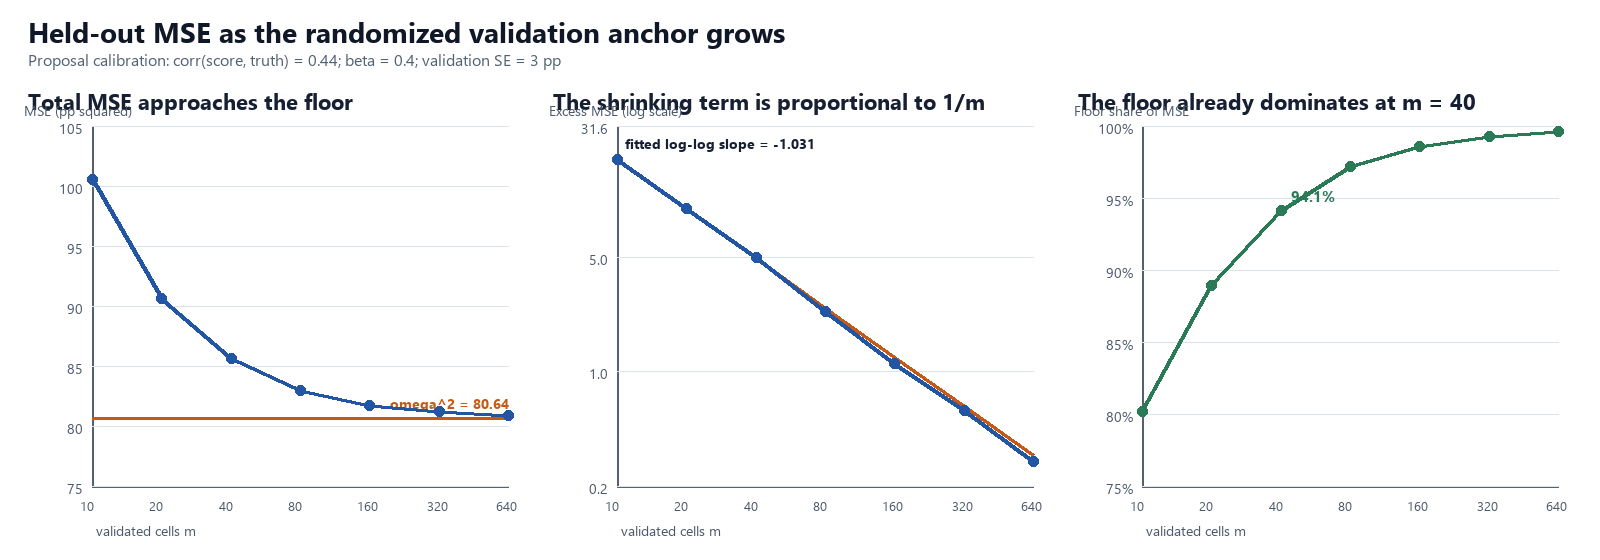
\includegraphics[width=\linewidth]
 {ai_mse_simulation_primary_2026-08-04.png}
 \caption{Held-out-cell MSE, its excess above the oracle floor, and the
 floor's share of total MSE. The plot is generated by the archived simulation
 code with the calibration in \eqref{eq:calibration}.}
 \label{fig:simulation}
\end{figure}

At \(m=40\), the shrinking term is 5.013 while the floor is 80.64. Increasing
\(m\) from 40 to infinity reduces RMSE only from
\(\sqrt{85.653}=9.25\) to \(\sqrt{80.64}=8.98\) percentage points. Thus the
proposal's forty-cell benchmark is near the knee for learning the shared
channel, but it does not imply precise prediction of an unvalidated cell.

More generally, the floor dominates when
\begin{equation}
 \omega^2\gg\frac{\Lambda}{m},
 \qquad\text{equivalently}\qquad
 m\gg\frac{\Lambda}{\omega^2}.
 \label{eq:dominance-condition}
\end{equation}
Using \(\widehat\Lambda=196.7\), the fitted \(\Lambda/m\) term is below 10
percent of the floor at approximately \(m=25\). \emph{Derived from the fitted
simulation relation.}

The conclusion is not that \(\omega^2\) dominates for every possible
parameter vector. Its existence whenever \(\sigma_S^2>0\) is a feature of
the model. Its numerical dominance depends on \(\omega^2,\Lambda\), and
\(m\). Within the simulated sensitivity grid, however, it is robust:
\begin{center}
\begin{tabular}{r r r r r}
\hline
\(\rho\) & RCT SE & \(\omega^2\) & \(\Delta_{40}\) & Floor share \\
\hline
0.30 & 3 & 91.00 & 5.36 & 94.4\% \\
0.44 & 3 & 80.64 & 5.01 & 94.1\% \\
0.70 & 3 & 51.00 & 3.31 & 93.9\% \\
0.44 & 1 & 80.64 & 4.58 & 94.6\% \\
0.44 & 6 & 80.64 & 6.39 & 92.7\% \\
\hline
\end{tabular}
\end{center}
\emph{Simulation result.} Changing RCT precision changes the shrinking term,
not the score-only floor. Changing score quality changes the floor itself.
The table establishes robustness over these five choices, not over all
possible data-generating processes.

\section{What dominance implies for risk measurement and for
\texorpdfstring{\(\theta_j\)}{theta j}}

\subsection*{Notation}

\begin{longtable}{>{\raggedright\arraybackslash}p{0.24\linewidth}
                  >{\raggedright\arraybackslash}p{0.68\linewidth}}
\hline
Symbol & Meaning \\
\hline
\endfirsthead
\hline
Symbol & Meaning \\
\hline
\endhead
\(j,m\) & Held-out cell and number of validated cells. \\
\(\theta_j,S_j,\mathcal D_m,\psi_0\) & Held-out true gain, its score,
validation data from other cells, and the true shared parameter vector. \\
\(m_j,u_j,\omega^2\) & Oracle score-only mean, cell-specific residual, and
its variance. \\
\(\widehat\theta_{j,m},\mathcal R_m,\Delta_m,\Lambda\) & Fitted prediction,
total MSE, excess MSE, and its first-order coefficient. \\
\(\widehat{\mathcal R}_m,\widehat\omega^2,
\widehat\Delta_m\) & Estimators of total risk, the floor, and their
difference \(\widehat{\mathcal R}_m-\widehat\omega^2\). \\
\(K_R,K_\omega\) & Effective numbers of independent observations used to
estimate total risk and the floor. \\
\(z_{.975}\) & 97.5th percentile of the standard normal distribution,
approximately 1.96. \\
\(T_j\) & Any estimator of \(\theta_j\) based on the held-out cell's score
and the validation data. \\
\(O_p(\cdot),\longrightarrow_p\) & Order in probability and convergence in
probability. \\
\hline
\end{longtable}

\subsection*{The shrinking term is a small difference between large objects}

Suppose one tries to estimate the shrinking term by subtraction:
\begin{equation}
 \widehat\Delta_m
 =\widehat{\mathcal R}_m-\widehat\omega^2.
 \label{eq:subtraction-estimator}
\end{equation}
Then
\begin{equation}
 \widehat\Delta_m-\Delta_m
 =(\widehat{\mathcal R}_m-\mathcal R_m)
 -(\widehat\omega^2-\omega^2).
 \label{eq:subtraction-error}
\end{equation}
Under ordinary square-root rates,
\begin{equation}
 \widehat{\mathcal R}_m-\mathcal R_m=O_p(K_R^{-1/2}),
 \qquad
 \widehat\omega^2-\omega^2=O_p(K_\omega^{-1/2}).
 \label{eq:risk-estimation-rates}
\end{equation}
Because \(\Delta_m\asymp m^{-1}\), relative consistency of
\eqref{eq:subtraction-estimator} requires
\begin{equation}
 K_R^{-1/2}=o(m^{-1}),
 \qquad
 K_\omega^{-1/2}=o(m^{-1}),
\end{equation}
or
\begin{equation}
 K_R\gg m^2,
 \qquad
 K_\omega\gg m^2.
 \label{eq:m-squared-requirement}
\end{equation}
\emph{Derived.} If \(\omega^2\) is estimated from the same \(m\) validation
cells, its ordinary error is \(O_p(m^{-1/2})\), which is larger than the
\(O(m^{-1})\) object being recovered. Direct subtraction therefore cannot
isolate \(\Lambda/m\) at relative precision without additional structure or
a cancellation-based estimator.
Indeed, ignoring the total-risk error only makes the problem easier, yet
\begin{equation}
 m(\widehat\Delta_m-\Delta_m)
 =-m(\widehat\omega^2-\omega^2)
 =O_p(\sqrt m),
 \label{eq:scaled-subtraction-error}
\end{equation}
which grows rather than vanishes. \emph{Derived under the ordinary
square-root rate for \(\widehat\omega^2\).}

An optimistic Gaussian calculation makes the scale concrete. If
\(\omega^2\) is known and \(K_R\) independent, mean-zero Gaussian prediction
errors have variance \(\mathcal R_m\), then the standard error of their mean
squared error is approximately
\(\sqrt{2}\mathcal R_m/\sqrt{K_R}\). Detecting \(\Delta_m\)
at the 95 percent normal threshold requires
\begin{equation}
 K_R
 \geq
 2z_{.975}^2
 \left(\frac{\mathcal R_m}{\Delta_m}\right)^2.
 \label{eq:detection-count}
\end{equation}
For the primary simulation this gives:
\begin{center}
\begin{tabular}{r r r r}
\hline
\(m\) & \(\Delta_m\) & \(\omega^2/\Delta_m\) & Required \(K_R\) \\
\hline
40  & 5.013 & 16.1  & 2,243 \\
80  & 2.331 & 34.6  & 9,732 \\
160 & 1.129 & 71.4  & 40,290 \\
320 & 0.579 & 139.2 & 150,980 \\
\hline
\end{tabular}
\end{center}
\emph{Derived from the Gaussian variance of a squared error and the simulated
risks.} Dependence across cells or estimation of \(\omega^2\) would increase
the requirement.

The simulation detected the rate with 2,000 repetitions because it knew the
simulated \(\omega^2\) and used the integrated expression
\eqref{eq:integrated-excess}. It did not recover a small unknown difference
by subtracting two noisy empirical MSE estimates. This distinction is
necessary before carrying the result to real data.

\subsection*{An unvalidated cell effect is not consistently estimable}

The word \emph{cell} is important. The proposal defines \(\theta_j\) as the
productivity gain in occupation-task cell \(j\). It is a cell-average causal
effect, not an individual worker's treatment effect. The question here is
whether the realized effect of one particular unvalidated cell can be
estimated precisely. \emph{Source: proposal, pp.~1--2.}

The stronger problem concerns \(\theta_j\) itself. From
\eqref{eq:residual},
\begin{equation}
 \widehat\theta_{j,m}-\theta_j
 =(\widehat\theta_{j,m}-m_j)-u_j.
 \label{eq:individual-error}
\end{equation}
Under the regularity conditions behind \eqref{eq:main-expansion},
\begin{equation}
 \widehat\theta_{j,m}-m_j=O_p(m^{-1/2}),
\end{equation}
so
\begin{equation}
 \widehat\theta_{j,m}-\theta_j
 =-u_j+O_p(m^{-1/2}).
 \label{eq:nonconvergence}
\end{equation}
If \(\omega^2>0\), the right side does not converge to zero. Therefore
\begin{equation}
 \widehat\theta_{j,m}\not\longrightarrow_p\theta_j,
 \qquad
 \MSE(\widehat\theta_{j,m})\longrightarrow\omega^2.
 \label{eq:not-consistent}
\end{equation}
\emph{Derived.}

This is not a defect of the plug-in estimator. If \(T_j\) is any estimator
measurable with respect to \((S_j,\mathcal D_m)\), conditional variance
decomposition gives
\begin{align}
 \E[(T_j-\theta_j)^2]
 &=\E[(T_j-\E[\theta_j\mid S_j,\mathcal D_m])^2] \\
 &\quad+\E[\Var(\theta_j\mid S_j,\mathcal D_m)] \\
 &\geq\E[\Var(\theta_j\mid S_j,\mathcal D_m)].
 \label{eq:bayes-lower-bound}
\end{align}
As the shared parameter becomes known, the last term converges to
\(\omega^2\). The posterior mean attains the lower bound. No other estimator
using the same information can remove it. \emph{Derived from conditional
variance decomposition and held-out-cell independence.}

Under the primary Gaussian calibration, the limiting posterior standard
deviation is 8.98 percentage points. A score-only 95 percent posterior
interval has approximate half-width
\begin{equation}
 1.96\sqrt{\omega^2}=17.6
 \label{eq:interval-width}
\end{equation}
percentage points. The simulation therefore reflects the mathematical
identification problem directly: after the \(1/m\) component becomes small,
almost all remaining prediction error is uncertainty about the particular
held-out cell.

\subsection*{The exact identification mistake in the proposal}

The proposal correctly distinguishes the shared score-to-truth channel from
the cell effects when it writes down the model. The mistake occurs when it
passes from identifying the shared channel to claiming recovery of the
realized map. Page~2 says that the validation pairs identify the common
score-to-truth channel and that empirical Bayes will ``recover the map.''
Appendix~A.2 is titled ``The randomized anchor identifies everything.'' The
Figure~1 caption similarly says that the calibrated estimates ``recover the
real structure of who gains.'' \emph{Source: proposal, pp.~1--2 and p.~4.}

Write the shared parameter vector as
\begin{equation}
 \psi_0=(\mu,\tau^2,a,b,\sigma_S^2).
 \label{eq:shared-parameter-vector}
\end{equation}
The randomized validation cells can consistently estimate this common
vector under the proposal's model:
\begin{equation}
 \widehat\psi_m\longrightarrow_p\psi_0.
 \label{eq:shared-parameter-consistency}
\end{equation}
The corresponding plug-in rule therefore satisfies
\begin{align}
 \widehat\theta_{j,m}
 &=h(S_j;\widehat\psi_m) \\
 &\longrightarrow_p h(S_j;\psi_0)
 =\E[\theta_j\mid S_j,\psi_0]
 =m_j.
 \label{eq:oracle-not-truth}
\end{align}
\emph{Derived under M1--M4 in Appendix~A.}

The invalid implication is
\begin{equation}
 \widehat\psi_m\longrightarrow_p\psi_0
 \quad\not\Longrightarrow\quad
 \widehat\theta_{j,m}\longrightarrow_p\theta_j.
 \label{eq:invalid-implication}
\end{equation}
Identifying \(\psi_0\) identifies the conditional distribution of
\(\theta_j\) given \(S_j\), including its posterior mean. It does not reveal
the realized residual \(u_j=\theta_j-m_j\). Because
\(\Var(u_j\mid S_j,\psi_0)=\omega^2>0\), different values of \(\theta_j\)
remain compatible with the same observed score even after the common channel
is known exactly. \emph{Derived from
\eqref{eq:oracle-variance}--\eqref{eq:residual}.}

Appendix~A.3 is not wrong when it states that the feasible estimator's
\emph{excess risk over the oracle} is
\(\Lambda/m+o(m^{-1})\). The interpretation becomes incorrect if that
excess-risk result is treated as a total-error result. The two statements are
\begin{align}
 \mathcal R_m-\omega^2
 &=\frac{\Lambda}{m}+o(m^{-1}),
 \label{eq:proposal-excess-risk}\\
 \mathcal R_m
 &=\omega^2+\frac{\Lambda}{m}+o(m^{-1}).
 \label{eq:proposal-total-risk}
\end{align}
Only the first difference converges to zero. \emph{The first rate is a
proposal claim; the second equality is derived from that claim and
\eqref{eq:main-decomposition}.}

Thus Appendix~A.2's phrase ``identifies everything'' is correct only if
``everything'' means the shared parameters and the posterior rule. It is
incorrect if it includes the realized vector
\((\theta_1,\ldots,\theta_J)\), the realized effect of an unvalidated cell,
or the exact true ranking of cells. The model identifies posterior means,
intervals, and ranking probabilities. It does not point-identify those
latent realizations. Aggregate quantities may nevertheless be precise when
many independent cell residuals average out, but that is a different
asymptotic argument and does not imply precise recovery of each cell.
\emph{Derived from \eqref{eq:bayes-lower-bound} and the distinction between
cell-level and aggregate error.}

The proposal therefore contains a mismatch rather than an error in the
displayed \(m^{-1}\) formula. Its formal result establishes convergence to
the score-only oracle, while its phrases ``recover the map'' and ``identifies
everything'' suggest convergence to the realized truth. If precise recovery
of every unvalidated \(\theta_j\) is the intended deliverable, the current
information structure cannot deliver it. A correct statement would say that
the validation anchor consistently estimates the common calibration channel
and produces a posterior distribution for each unvalidated cell, with
limiting conditional variance \(\omega^2\).

\section{What can reduce the cell-level floor}

\subsection*{Notation}

\begin{longtable}{>{\raggedright\arraybackslash}p{0.24\linewidth}
                  >{\raggedright\arraybackslash}p{0.68\linewidth}}
\hline
Symbol & Meaning \\
\hline
\endfirsthead
\hline
Symbol & Meaning \\
\hline
\endhead
\(j,m,J,R_j\) & Cell index, validation count, total cells, and validation
indicator. \\
\(\theta_j,S_j,\widehat v_j,s_j^2\) & True gain, broad score, direct RCT
estimate, and its error variance. \\
\(\tau^2,a,b,\rho,\psi_0,\omega^2\) & Cross-cell variance, score intercept
and slope, score-truth correlation, true shared parameter, and current
score-only floor. \\
\(\Delta_m\) & Shared-parameter component of held-out MSE. \\
\(\ell=1,\ldots,n_j\) & Cheap score observation and number of such
observations in cell \(j\). \\
\(S_{j\ell},\bar S_j\) & Conversation-level score and its cell average. \\
\(B_j,\sigma_B^2\) & Systematic cell-level score error and its variance. \\
\(e_{j\ell},\bar e_j,\sigma_e^2\) & Idiosyncratic score error, its cell
average, and its variance. \\
\(\omega_j^2(n_j)\) & Posterior variance after averaging \(n_j\) cheap score
observations. \\
\(Z_j,\zeta_j,q_j^2\) & Additional cheap causal measurement for cell \(j\),
its error, and its error variance. \\
\(X_j,\omega_X^2\) & Additional cell characteristics and the remaining
conditional variance after using them. \\
\(r_\star\) & Desired score-only RMSE for an unvalidated cell. \\
\(\operatorname{RMSE}\) & Root mean squared error. \\
\hline
\end{longtable}

For a validated cell in the primary calibration, \eqref{eq:validated-variance}
gives
\begin{equation}
 \Var(\theta_j\mid S_j,\widehat v_j,\psi_0)
 =\frac{80.64(9)}{80.64+9}=8.10,
 \qquad
 \operatorname{RMSE}=2.85.
 \label{eq:validated-numeric}
\end{equation}
\emph{Derived.} The direct measurement therefore changes cell-level
precision materially. But with \(m=40\) and \(J=1{,}000\), only 4 percent of
cells receive it; 96 percent remain score-only under the basic design.

The project already has cheap data for every cell through \(S_j\). The first
question is therefore not whether another broad score exists. It is whether
the error in the existing score averages away as the number of conversations
in the cell grows.

To separate sampling error from systematic cell error, write
\begin{equation}
 S_{j\ell}=a+b\theta_j+B_j+e_{j\ell},
 \qquad
 \bar S_j=a+b\theta_j+B_j+\bar e_j,
 \label{eq:repeated-score-model}
\end{equation}
with mutually independent Gaussian components for this diagnostic model,
\begin{equation}
 \Var(B_j)=\sigma_B^2,
 \qquad
 \Var(e_{j\ell})=\sigma_e^2.
 \label{eq:score-components}
\end{equation}
Then
\begin{equation}
 \omega_j^2(n_j)
 =\left[
 \frac1{\tau^2}
 +\frac{b^2}{\sigma_B^2+\sigma_e^2/n_j}
 \right]^{-1}.
 \label{eq:repeated-score-variance}
\end{equation}
\emph{Derived under the diagnostic Gaussian model.}

If \(\sigma_B^2=0\), then
\(\omega_j^2(n_j)\to0\): enough cheap observations can identify
\(\theta_j\) precisely. If \(\sigma_B^2>0\), then
\begin{equation}
 \omega_j^2(n_j)
 \longrightarrow
 \left(\frac1{\tau^2}+\frac{b^2}{\sigma_B^2}\right)^{-1}>0.
 \label{eq:systematic-floor}
\end{equation}
More conversations remove \(e_{j\ell}\) but not \(B_j\). The immediate
empirical task is therefore to estimate whether validation residual variance
falls with cell interaction counts or instead plateaus. Repeated scoring and
independent scoring methods can also separate transient variation from
shared systematic error. \emph{Design implication.}

Improving the score can solve the problem only if it is substantial in the
real data. From \(\omega^2=\tau^2(1-\rho^2)\), attaining a desired score-only
RMSE \(r_\star\) requires
\begin{equation}
 \rho\geq\sqrt{1-\frac{r_\star^2}{\tau^2}}.
 \label{eq:required-correlation}
\end{equation}
With \(\tau=10\), the requirements are:
\begin{center}
\begin{tabular}{r r}
\hline
Desired \(r_\star\) & Required \(\rho\) \\
\hline
5 percentage points & 0.866 \\
3 percentage points & 0.954 \\
2 percentage points & 0.980 \\
\hline
\end{tabular}
\end{center}
\emph{Derived.} A favorable correlation chosen only inside a simulation is
not a fix; the observed score must actually attain that reliability.

If the existing score retains systematic error, four changes are possible.

\begin{enumerate}[label=\arabic*.,leftmargin=2.2em]
 \item \textit{Improve the cell-specific predictors.} Add measured task
 complexity, baseline duration, verifiability, workflow, user composition,
 and other characteristics \(X_j\). The new floor is
 \begin{equation}
  \omega_X^2
  =\E[\Var(\theta_j\mid S_j,X_j)].
  \label{eq:x-floor}
 \end{equation}
 This helps only if the conditional residual variance actually falls on
 held-out validation cells. A flexible prediction method cannot remove a
 cell-specific residual that its inputs do not measure.

 \item \textit{Give important cells a cheap causal signal.} A broad platform
 randomization or randomized rollout could yield
 \begin{equation}
  Z_j=\theta_j+\zeta_j,
  \qquad
  \Var(\zeta_j)=q_j^2.
  \label{eq:cheap-causal-signal}
 \end{equation}
 Combining it with the calibrated score gives
 \begin{equation}
  \Var(\theta_j\mid S_j,Z_j)
  =\left(\frac1{\omega^2}+\frac1{q_j^2}\right)^{-1}.
  \label{eq:cheap-causal-variance}
 \end{equation}
 This is an additional cell-specific causal measurement, not another copy of
 the existing \(S_j\). When universal randomization is infeasible, scarce
 experimental observations can be allocated toward cells with the largest
 posterior uncertainty or greatest decision value. This improves those cells;
 it does not identify a cell that still receives no new information.

 \item \textit{Impose and test shared structure.} Occupation-by-task effects
 may have a low-dimensional or low-rank structure. Experiments in selected
 cells could then reveal components shared with an unvalidated cell. This
 replaces the exchangeable random-effects model with a stronger restriction.
 It is useful only to the extent that held-out-cell residuals from that
 structure are small; otherwise a new floor remains.

 \item \textit{Use credible quasi-experimental variation.} Staggered rollout,
 eligibility rules, capacity constraints, or randomized encouragement can
 provide cell-specific treatment variation without a separate enterprise RCT.
 The resulting estimate is causal only under the assumptions appropriate to
 that source of variation; ordinary observational prediction is not a
 substitute.

 \item \textit{Change the reported estimand or precision claim.} If neither
 cell-specific causal information nor a well-supported predictive structure
 is available, report posterior means with their full intervals, or report
 effects for broader occupation or task groups. Pooling can identify a group
 mean more precisely, but it does not identify the original individual
 \(\theta_j\).
\end{enumerate}

Changing the simulation parameters can illustrate when the problem is large
or small. It is not a substantive fix unless the real data become more
informative. Increasing \(m\), improving the RCT precision in other cells, or
changing the empirical-Bayes estimator reduces \(\Delta_m\); none of these
changes eliminates \(\omega^2\) for a cell that still supplies only the same
noisy \(S_j\).

\appendix

\section{Derivation of the held-out-cell MSE}

\subsection*{Notation}

\begin{longtable}{>{\raggedright\arraybackslash}p{0.24\linewidth}
                  >{\raggedright\arraybackslash}p{0.68\linewidth}}
\hline
Symbol & Meaning \\
\hline
\endfirsthead
\hline
Symbol & Meaning \\
\hline
\endhead
\(j,m,R_j\) & Held-out cell, validation count, and validation indicator. \\
\(\theta_j,S_j,\eta_j,\widehat v_j,\varepsilon_j\) & True gain, score,
score error, validation estimate, and validation error. \\
\(\mu,\tau^2,a,b,\sigma_S^2\) & The five shared Gaussian channel
parameters. \\
\(\psi,\psi_0,\widehat\psi_m\) & Generic, true, and estimated shared
parameter vectors, ordered as \((\mu,\tau^2,a,b,\sigma_S^2)\). \\
\(\mathcal D_m,h,m_j,\widehat\theta_{j,m}\) & Validation data,
conditional-mean rule, oracle score-only mean, and fitted prediction. \\
\(\mathcal R_m,\omega^2,\Lambda\) & Total held-out MSE, oracle floor, and
coefficient on \(m^{-1}\). \\
\(\dot h(S_j;\psi_0)\) & Derivative of \(h\) with respect to \(\psi\). \\
\(V_\psi\) & Asymptotic second-moment matrix of
\(\sqrt m(\widehat\psi_m-\psi_0)\). \\
\(r_{j,m}\) & Remainder in the first-order Taylor expansion. \\
\(D_S,x_j\) & Score variance \(b^2\tau^2+\sigma_S^2\) and centered score
\(S_j-a-b\mu\). \\
\(\lambda\) & Score reliability ratio
\(b^2\tau^2/(b^2\tau^2+\sigma_S^2)\). \\
\(s^2,\widehat\mu_m\) & Common validation-error variance and validation-mean
estimator in the final simple case. \\
\(o(m^{-1})\) & A term that is small relative to \(m^{-1}\). \\
\hline
\end{longtable}

The derivation uses four conditions.
\begin{enumerate}[label=\textup{M\arabic*},leftmargin=2.5em]
 \item The Gaussian model \eqref{eq:model} is correct.
 \item The held-out cell is not used to estimate the shared parameter:
 \begin{equation}
  \mathcal D_m\indep(\theta_j,S_j)\mid\psi_0.
  \label{eq:holdout}
 \end{equation}
 \item The shared-parameter estimator satisfies
 \begin{equation}
  \sqrt m(\widehat\psi_m-\psi_0)\Rightarrow N(0,V_\psi),
  \qquad
  m\E[(\widehat\psi_m-\psi_0)(\widehat\psi_m-\psi_0)^\top]
  \longrightarrow V_\psi.
  \label{eq:parameter-rate}
 \end{equation}
 \item The function \(h\) is differentiable at \(\psi_0\),
 \(\E[r_{j,m}^2]=o(m^{-1})\), and cross terms containing the remainder are
 \(o(m^{-1})\).
\end{enumerate}
M1 is the proposal's model. M2--M4 are additional assumptions. The proposal
does not state this complete set. \emph{Scope qualification.}

Add and subtract \(m_j=h(S_j;\psi_0)\):
\begin{equation}
 \widehat\theta_{j,m}-\theta_j
 =(m_j-\theta_j)+(\widehat\theta_{j,m}-m_j).
 \label{eq:error-split}
\end{equation}
Squaring and taking expectations gives
\begin{align}
 \mathcal R_m
 &=\E[(m_j-\theta_j)^2]
   +\E[(\widehat\theta_{j,m}-m_j)^2] \\
 &\quad+2\E[(m_j-\theta_j)(\widehat\theta_{j,m}-m_j)].
 \label{eq:three-terms}
\end{align}
The cross term is zero:
\begin{align}
 &\E[(m_j-\theta_j)(\widehat\theta_{j,m}-m_j)] \\
 &\quad=\E\!\left[
  (\widehat\theta_{j,m}-m_j)
  \E[m_j-\theta_j\mid S_j,\mathcal D_m,\psi_0]
 \right] \\
 &\quad=0.
 \label{eq:cross-zero}
\end{align}
The first equality is iterated expectation. The last equality uses M2 and
\(\E[\theta_j\mid S_j,\psi_0]=m_j\). Also,
\begin{align}
 \E[(m_j-\theta_j)^2]
 &=\E[\Var(\theta_j\mid S_j,\psi_0)] \\
 &=\omega^2.
 \label{eq:omega-term}
\end{align}
Substitution proves the exact decomposition
\begin{equation}
 \mathcal R_m
 =\omega^2+
 \E[\{h(S_j;\widehat\psi_m)-h(S_j;\psi_0)\}^2].
 \label{eq:exact-mse}
\end{equation}
\emph{Derived from M1--M2.}

By M3--M4,
\begin{equation}
 h(S_j;\widehat\psi_m)-h(S_j;\psi_0)
 =\dot h(S_j;\psi_0)^\top(\widehat\psi_m-\psi_0)+r_{j,m}.
 \label{eq:taylor}
\end{equation}
Using M2 to separate the held-out score from the validation estimator,
\begin{align}
 &\E[\{h(S_j;\widehat\psi_m)-h(S_j;\psi_0)\}^2] \\
 &\quad=\frac1m
 \E[\dot h(S_j;\psi_0)^\top V_\psi\dot h(S_j;\psi_0)]
 +o(m^{-1}) \\
 &\quad=\frac{\Lambda}{m}+o(m^{-1}),
 \label{eq:estimated-parameter-error}
\end{align}
where
\begin{equation}
 \Lambda
 =\E[\dot h(S_j;\psi_0)^\top V_\psi\dot h(S_j;\psi_0)].
 \label{eq:lambda-definition}
\end{equation}
Substitution into \eqref{eq:exact-mse} proves
\begin{equation}
 \mathcal R_m
 =\omega^2+\frac{\Lambda}{m}+o(m^{-1}).
 \label{eq:final-mse}
\end{equation}
\emph{Derived from M1--M4.}

For completeness, let
\begin{equation}
 D_S=b^2\tau^2+\sigma_S^2,
 \qquad
 x_j=S_j-a-b\mu.
\end{equation}
Direct differentiation of \eqref{eq:oracle-mean} gives
\begin{equation}
 \dot h(S_j;\psi_0)
 =
 \begin{pmatrix}
 \displaystyle \frac{\sigma_S^2}{D_S}\\[0.65em]
 \displaystyle \frac{b\sigma_S^2x_j}{D_S^2}\\[0.65em]
 \displaystyle -\frac{b\tau^2}{D_S}\\[0.65em]
 \displaystyle
 \frac{\tau^2(\sigma_S^2-b^2\tau^2)x_j}{D_S^2}
 -\frac{b\tau^2\mu}{D_S}\\[0.65em]
 \displaystyle -\frac{b\tau^2x_j}{D_S^2}
 \end{pmatrix}.
 \label{eq:gradient}
\end{equation}
The rows follow the order
\((\mu,\tau^2,a,b,\sigma_S^2)\). Hence \(\Lambda\) is determined once the
validation design determines \(V_\psi\). \emph{Derived.}

A simple case makes the \(m^{-1}\) term transparent. Suppose \(\mu\) is the
only unknown shared parameter and
\begin{equation}
 \widehat\mu_m=\frac1m\sum_{j:R_j=1}\widehat v_j,
 \qquad
 \Var(\varepsilon_j)=s^2,
\end{equation}
with independent validation cells and errors. Then
\begin{equation}
 \Var(\widehat\mu_m)=\frac{\tau^2+s^2}{m},
 \qquad
 \frac{\partial h}{\partial\mu}
 =\frac{\sigma_S^2}{b^2\tau^2+\sigma_S^2}
 =1-\lambda.
\end{equation}
The formula is exact in this case:
\begin{equation}
 \mathcal R_m
 =\omega^2+
 \frac{(1-\lambda)^2(\tau^2+s^2)}{m}.
 \label{eq:special-case}
\end{equation}
\emph{Derived.}

\section*{Conclusion}

The broad score \(S_j\) is observed in every cell. The randomized anchor
learns how that score relates to true gains, and the simulation confirms that
its shared-parameter error falls approximately as \(1/m\). Under the proposal
calibration, that error is already small near \(m=40\); almost all remaining
held-out-cell MSE is \(\omega^2\).

The existence of a positive floor comes from the current score-plus-random-
anchor model. Its numerical dominance is parameter-dependent. When it
dominates, an unvalidated \(\theta_j\) is not merely difficult to estimate:
it is not consistently estimable from \((S_j,\mathcal D_m)\). A defensible
fix must show that repeated cheap score data remove the score error, add
cell-specific information, impose a validated structure that makes the
residual small, or weaken the cell-level precision claim.

This establishes the proposal's exact overreach. The randomized anchor can
identify the shared channel and make the feasible predictor approach the
oracle. It cannot, under the same information structure, make that oracle
equal the realized effect in an unvalidated cell.

\end{document}
